%!TEX root = ../main.tex

\subsection*{Ejercicio 4.}
Al aproximar una función continua $f : [0, 1] \to \mathbb{R}$ mediante un polinomio $p(t) = a_n t^n + \cdots + a_1 t + a_0$, el error de aproximación $E$ se mide en la norma $L^2$, es decir:
\[
E^2 := \|p - f\|_{L^2}^2 = \int_0^1 [p(t) - f(t)]^2 \, dt.
\]

\begin{enumerate}
    \item[(a)] Muestre que la minimización del error $E = E(a_0, \ldots, a_n)$ conduce a un sistema de ecuaciones lineales $H_n a = b$, donde:
    \[
    b = [b_0, \ldots, b_n]^T \in \mathbb{R}^{n+1}, \quad b_i = \int_0^1 f(t)t^i \, dt, \quad i = 0, \ldots, n,
    \]
    y $H_n$ es la matriz de Hilbert de orden $n$, definida como:
    \[
    (H_n)_{i,j} = \frac{1}{i + j + 1}, \quad i, j = 0, \ldots, n.
    \]
    El vector $a$ representa los coeficientes del polinomio $p$.\\

    \begin{proof}
    Sea $p(t)=\displaystyle\sum_{j=0}^{n} a_jt^j$, note que 

    \begin{align*}
        E^2(a_0,\ldots,a_n)&=\int_0^1\left(p(t)-f(t)\right)^2dt\\
        &=\int_0^1\left(\sum_{j=0}^{n} a_jt^j-f(t)\right)^2dt\\
        &=\int_0^1\left(\sum_{j=0}^{n} a_jt^j\right)^2dt-2\int_0^1f(t)\sum_{j=0}^{n} a_jt^j dt+\|f\|_{L^2}^2
    .\end{align*}

    Note que esta función depende de los coeficientes, por lo tanto para minimizar el error podemos derivar parcialmente con respecto a $a_k$, $0\leq k\leq n$ e igualar a 0. Derivando obtenemos que

    \begin{align*}
        \frac{\partial E^2}{\partial a_k}=2\int_0^1\left(\sum_{j=0}^{n} a_jt^{k+j}\right)dt-2\int_0^1f(t)t^kdt=0 
    ,\end{align*}
    
    despejando de esta ecuación obtenemos que

    $$\int_0^1\sum_{j=0}^{n} a_jt^{j+k}dt=\sum_{j=0}^{n} a_j\int_0^1t^{j+k}dt=\int_0^1f(t)t^k dt,$$

    más aún, como $\displaystyle\int_0^1t^{k+j}dt=\frac{1}{k+j+1}=(H_n)_{k,j}$, obtenemos

    $$\sum_{j=0}^{n} a_j(H_n)_{k,j}=(H_n)_k\begin{pmatrix}
           a_{1} \\
           a_{2} \\
           \vdots \\
           a_{n}
         \end{pmatrix}=\int_0^1f(t)t^kdt=b_k,$$

donde $(H_n)_k$ denota la $k-$ésima fila de la matriz $(H_n)$, que es lo mismo que $H_n a=b$.


    \end{proof}

    \item[(b)] Muestre que $H_n$ es simétrica y definida positiva.\\

    \begin{proof}
    Note que la simetría es inmediata de  que

    $$(H_n)_{i,j}=\frac{1}{i+j+1}=\frac{1}{j+i+1}=(H_n)_{j,i}.$$

    Para ver que la matriz es definida positiva note que
    $$
\begin{aligned}
x^T H_n x & =\left(x_1, \ldots, x_n\right)\left(\begin{array}{ccc}
1 & \cdots & \dfrac{1}{n+2} \\
\vdots & \ddots & \vdots \\
\dfrac{1}{n+2} & \cdots & \dfrac{1}{2 n+1}
\end{array}\right)\left(\begin{array}{c}
x_1 \\
\vdots \\
x_n
\end{array}\right) \\
& =\sum_{i=0}^n \sum_{j=0}^n \frac{x_j x_i}{i+j+1} \\
& =\sum_{i=0}^n \sum_{j=0}^n x_j x_i \int_0^1 t^i t^j d t \\
& =\int_0^1 \sum_{i=0}^n x_i t^i \sum_{j=0}^n x_j t^j d t \\
& =\left\|\sum_{j=0}^{n} x_jt^j\right\|_{L^2}^2>0
\end{aligned}
$$
    \end{proof}

    \item[(c)] Solucione el sistema $H_n x = b$, donde $b$ tiene componentes $b_i = 1 / (n + i +1)$, para $i = 0, \ldots, n$. Para esto, use las factorizaciones LU ($[L, U] = \text{lu}(H)$) y Cholesky ($L = \text{chol}(H)$). Luego resuelva los dos sistemas triangulares.

    \begin{solution}
    El teorema de Stone-Weierstrass nos dice que los polinomios son densos en las funciones continuas, esto nos da que la aproximación que nos piden es posible, al truncar el número de coeficientes del polinomio vimos que el problema de optimizarlos se reduce a resolver el sistema $H_nx=b$, esto podemos programarlo en Matlab, Python, etc. Para este caso nosotros hemos hecho el trabajo en ambos lenguajes con el propósito de comparar resultados, antes de presentar los códigos en Matlab observemos que

    $$b_i=\dfrac{1}{n+i+1}=\int_0^1f(t)t^i dt,$$

    y por lo tanto $f(t)=t^n$, en efecto estamos aproximando el polinomio $t^n$ por polinomios, así pues, esperaríamos una solución numérica del estilo $a=(0,\ldots,1)^T$. Para el caso de la factorización $LU$ implementamos

    \begin{lstlisting}
    n = 10; 
    H = hilb(n); %Genera la matriz de Hilbert de orden n
    b = zeros(n, 1); %Crea un vector con n ceros 
    for i = 1:n
        b(i) = 1 / (i + n - 1); %Cambia  las entradas por las del ejercicio
    end
    [L, U] = lu(H);

    %Solucionamos los sistemas

    y = L \ b;
    a_LU = U \ y;

    disp(a_LU')
    \end{lstlisting}

    En el caso de la factorización de Cholesky

    \begin{lstlisting}
    n = 10; 
    H = hilb(n); 
    b = zeros(n, 1); 
    for i = 1:n
        b(i) = 1 / (i + n - 1); 
    end
    L = chol(H); 
    y = L' \ b;
    a_LU = L \ y;
    disp(a_LU')
    \end{lstlisting}

    En ambos casos tomamos un tamaño $n=10$ para probar el algoritmo, en donde la factorización $LU$ nos arrojó el resultado $x=(0,0,0,0,0,0,0,0,0,1)^T$ y la factorización de Cholesky nos dió el resultado 

   \[x=
\begin{bmatrix}
4.4438 \times e^{-11} \\
-3.8598 \times e^{-9} \\
8.2505 \times e^{-8} \\
-7.5194 \times e^{-7} \\
3.5931 \times e^{-6} \\
-9.8904 \times e^{-6} \\
1.6243 \times e^{-5} \\
-1.5708 \times e^{-5} \\
8.2514 \times e^{-6} \\
1
\end{bmatrix}
\]
    \end{solution}

    \item[(d)] Para ambos métodos, ¿qué tan precisas son las soluciones numéricas $\hat{x}_{\text{approx}}$? Tabule los errores de la solución:
    \[
    e(n) = \|\hat{x}_{\text{approx}} - x_{\text{exact}}\|
    \]
    como una función de $n = 2, \ldots, 15$. Note que $x_{\text{exact}} = (0, \ldots, 1)^T$. Puede graficar los errores en función de $n$ utilizando la función \texttt{semilogy} de Matlab. Explique en detalle los resultados.
\end{enumerate}

\begin{solution}
Implementamos el código en Matlab y obtuvimos los siguientes resultados para \\$n\leq 13$,

\begin{center}
    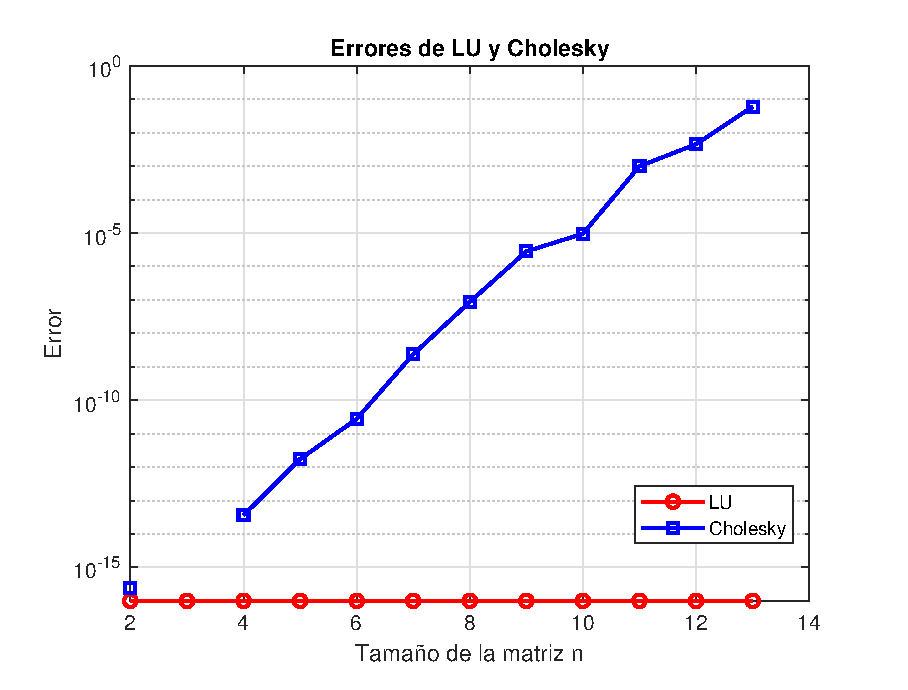
\includegraphics[scale=0.7]{Graficas/tarea_2_coya.eps}
\end{center}

cuando $n \geq 14$ Matlab falla al realizar Cholesky, detecta que la matriz de Hilbert no es definida positiva, pero ya demostramos que sí lo es, esto ocurre ya que el número de condición de la matriz de Hilbert crece  rápidamente confirme el tamaño de la matriz aumenta, como se evidencia en la siguiente figura

\begin{center}
    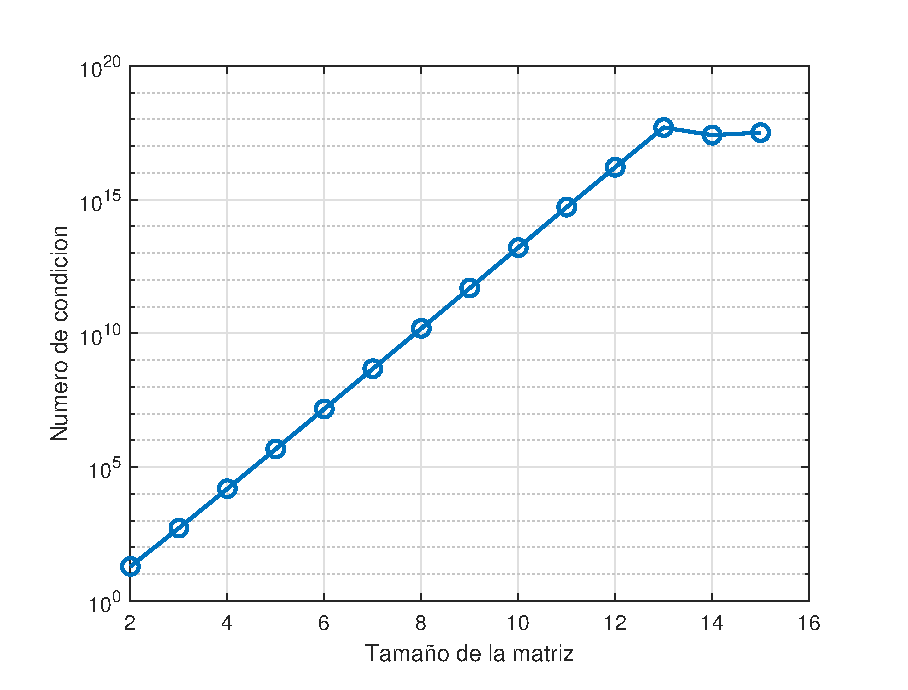
\includegraphics[scale=0.7]{Graficas/condicion_tarea2.eps}
\end{center}

por ejemplo para $n=6$ tenemos que $\mathcal{K}(H)>10^5$, esto en el método de Cholesky genera inconvenientes dado que la matriz debe ser definida positiva, como el método de factorización LU no tiene esta restricción entonces es más estable numéricamente para estos valores. El código usado para grafica el número de condición lo adjuntamos también en el cuaderno de Jupyter.

\end{solution}